\documentclass[]{article}
\usepackage{amssymb}
\usepackage{amsmath}
\usepackage{graphicx}
\usepackage{amsthm}
\newtheorem{theorem}{Theorem}

% Title Page
\title{Entry Guidance for Propellant Optimal Powered Descent on Mars}
\author{Connor Noyes}


\begin{document}
\maketitle

\section{Notes}
 N-dimensional interpolation is possible offline, but may be problematic online. A structured grid might alleviate the problem if enough samples can be generated 
In this analytical MPC approach, the propellant consumed is managed by the triggering mechanism. 

Different from standard MPC since the entire trajectory in planned, not a receding horizon. More of a shrinking horizon?

Due to the high velocity at which SRP begins, the onboard knowledge of the vehicle's state may not be well known. As the vehicle decelerates, the estimate will become better and a ground-relative nav solution is obtained. From this info, the final landing site, which may be different than the nominal landing site, is determined. The vehicle budgets propellant for the nominal target (it has to aim somewhere at ignition) as well as a separate allotment for any divert maneuver.

%For a constant, maximal thrust, the optimal range to go and altitude at ignition for a variety of velocity/fpa combos can be found very easily. This is the target manifold for the entry guidance termination. The manifold is `finite' since the propellant onboard is limited. Essentially, we have removed the positional states from the SRP problem, and relegated them to the entry phase. 

%It appears to be the case that only the magnitude of the velocity determines the propellant cost, while the optimal altitude/distance depends on the flight path angle. Update: this depends on the constants g0, Tmax, Isp. 

Small range error is not generally an issue because the vertical descent portion can do a divert if needed, and one may be needed even at the nominal landing site. 

Should start checking for ignition at the highest velocity at which it would be possible to land with the allotted propellant. 

%The switching curve in 1-D is now a manifold that the spacecraft may not reach; desired to ignite at minimal distance from the manifold. 

Any adaptive triggering mechanism must make use of some form of prediction to determine if the current state is suitable for triggering, and if the condition is improving or not. So long as the vehicle is decelerating, the velocity state is improving. However, the positional states may or may not be improving, e.g., if the optimal downrange distance is overshot. Thus, triggering should occur either when 
\begin{itemize}
\item The vehicle's altitude is too low and SRP must begin to achieve a soft landing 
\item the down range distance to the target has become too short and prolonging further will incur additional downrange error
\item The vehicle begins to accelerate because drag (velocity) has dropped too low while the flight path angle has become steep 
\end{itemize}

concerning entry guidance, do altitude optimal trajectories at a fixed velocity have the same characteristics as minimal velocity trajectories at a fixed final altitude?

Any derivation involving a change in mass cannot be decoupled 

%Ought to compare the derived terminal manifold with that obtained by assuming a constant mass. 

Draw diagram explaining the difference between range control and srp control

%Formal neighboring optimal control would minimize velocity subject to that terminal constraint 

\section{Notes and Observations}
A constant lift up bank angle is in fact optimal for maximal altitude at a fixed velocity (or minimal velocity at a fixed altitude) if the entry flight path angle is free and the downrange distance is free as well (fixed at zero crossrange). If the downrange distance is not the optimal one (for a given flight path angle)

The entry flight path angle is probably generally determined based on constraints like heat rate, total heat load, or g-load. Might still be able to choose between a range. 

As the vehicle flies, the estimated SRP propellant required from the current state may not be monotonic. But the estimated propellant required from the optimal ignition point may be? 

\textbf{TODO:} Examine the shape of the objective function, very bowl shaped but with a fairly flat bottom. Consider framing the discussion in terms of invariant sets? 

\textbf{TODO:} Diagram showing full predicted entry trajectory, highlight the portion checked for SRP, show the ignition condition.

Given a downrange distance and site altitude, there will be a range of entry flight path angles that admit solutions for a given control parametrization, such as a constant bank angle with one reversal. Among these admissible flight paths, the optimal one in terms of propellant occurs at the steepest entry with the lowest bank angle. This of course has no robustness, as any disturbances that result in lower energy than the nominal case will fall short and be forced to fly a lengthened, suboptimal powered approach. 

In short, if a constraint such as g-limit, or total heat load, or maximum heat rate forces the entry flight path to lie in a certain range, there will be a corresponding family of trajectories with different SRP costs. If no solutions with sufficiently low propellant costs exist for the desired flight path range, it is possible the target downrange is not chosen suitably and must be changed, or potentially no trajectory exists with such a cost. 

\subsection{Entry State to SRP State Conversion}
Given an entry state of the form $[r,\, \theta,\, \phi,\, v,\, \gamma,\, \psi]$, the corresponding SRP state is found by assuming the current heading $\psi$ defines the downrange distance. For a fixed target $(h_T,\, \theta_T,\, \phi_T)$, the range to go, and crossrange to target are computed. The SRP state is given by $[rtg,\, |cr|,\, r-r_p-h_T, v\cos\gamma, 0, v\sin\gamma, m_0]$. First, note that the absolute value of the crossrange is used; this gives a denser table of tabulated solutions by exploiting symmetry. Similarly, because the downrange direction is defined by the heading angle, the cross track velocity is always zero, allowing the use of 5D interpolation rather than 6D, again allowing the same number of solutions to more densely cover the input space. 

\section{Intro}
Powered descent played a role on MSL, and will also be used in M2020, MSR/SRL campaign. In future missions, supersonic retropropulsion may be used to land larger, heavier vehicles than the current generation of landers, and powered descent will play an even more significant role in the EDL process. There exist many guidance approaches to the SRP problem, with many focusing on fuel optimality, including GFOLD and other convex optimization methods, polynomial guidance, indirect methods, etc. In brief, there is no shortage of ways to tackle the problem of decelerating via propulsion. 

Far less attention has been given to the problem of entry guidance targeting favorable SRP ignition conditions. The only such work (by Ping Lu) has several areas for improvement. 

An adaptive trigger for termination of unguided flight was demonstrated to provide massive benefits over triggering at a fixed state (downrange, velocity, energy). The issue of monotonicity was dealt with by solving a related SRP problem. Despite presenting a predictor-corrector approach in which a prediction of the terminal entry state is available and being used to module the bank angle, only the current state is checked for triggering. Our approach to the triggering mechanism differs in that we utilize the prediction. This allows us to skirt the issue of monotonicity of predicted fuel consumption, and also guarantees we find the global minimum. 

Another issue is the role of bank angle modulation, and the chosen parametrization of the bank angle. In the work by Ping Lu, the bank angle is still modulated to perform range control, and utilizes a profile linear in energy with one parameter. 

A fundamental difference from parachute-based EDL architectures, even those that still utilize a vertical descent phase with potential for a divert maneuver prior, is in the desirable states at the termination of the entry phase. Traditionally, the entry objective is range control with lateral control as a secondary objective, and the two can be neatly decoupled. In determining the SRP ignition state, however, both the lateral and longitudinal motion is required. 

Additionally, the entry guidance approach utilizes knowledge of the planned SRP guidance approach, making the two phases linked by more than just the adaptive trigger because the bank angle is actively modulated to reduce predicted fuel consumption. 

An outline of the algorithmic approach, given a fixed bank angle parametrization and a pre-specified powered descent guidance method, is 
\begin{enumerate}
\item Integrate the estimated vehicle state forward using the current bank angle parametrization until the target altitude is reached
\item Determine the optimal ignition state along the powered descent trajectory
\item If the estimated optimal fuel consumption is unacceptable, update the bank angle profile parameters to optimize 
\end{enumerate}


\section{Entry Guidance Details}
%\begin{list}
%Delivery errors are handled via replanning
%Lift, drag, density disturbances via L/D control? Tracking?
%\end{list}


\subsection{Bank Angle Parametrizations}
Two different parametrizations of the bank angle profile were tested. Each is a two-parameter profile designed to generate both longitudinal and lateral motion. The first is a constant bank angle $\sigma_c$ with one reversal at a velocity $v_r$
\begin{equation}
\sigma(v) = \left\{
\begin{array}{ll}
\sigma_c & v\geq v_r \\
-\sigma_c & v\le v_r
\end{array} 
\right.
\end{equation}
while the second fixes the bank angle magnitudes and uses two reversal velocities $(v_1,\,v_2)$
\begin{equation}
\sigma(v) = \left\{
\begin{array}{ll}
\sigma_1 & v\geq v_1 \\
\sigma_2 & v_2\leq v\le v_1 \\
\sigma_3 & v< v_2
\end{array} 
\right.
\end{equation}
and we used $\sigma_1 = 90^\circ$, $-\sigma_2 = \sigma3 = 15^\circ$.
\subsection{Optimization}

\subsubsection{Objective Function}
The SRP problem admits continuous solutions, and the entry equations are also smooth for smooth bank angle inputs. Thus we expect that even when optimizing the ignition condition along a trajectory rather than use a fixed state variable such as velocity or energy, the objective function should be well behaved. One question is whether several isolated minima exist, or only a single global optimum. 

Evaluating the objective function for a range of parameters for each profile indicates the objective function is bowl shaped, potentially with a fairly flat both in the case of the second profile. The shape of the objective function means that gradient-based methods will be effective in determining the optimal profile parameters. 

\begin{figure}[h!]
	   \begin{minipage}{0.45\textwidth}
		\centering
		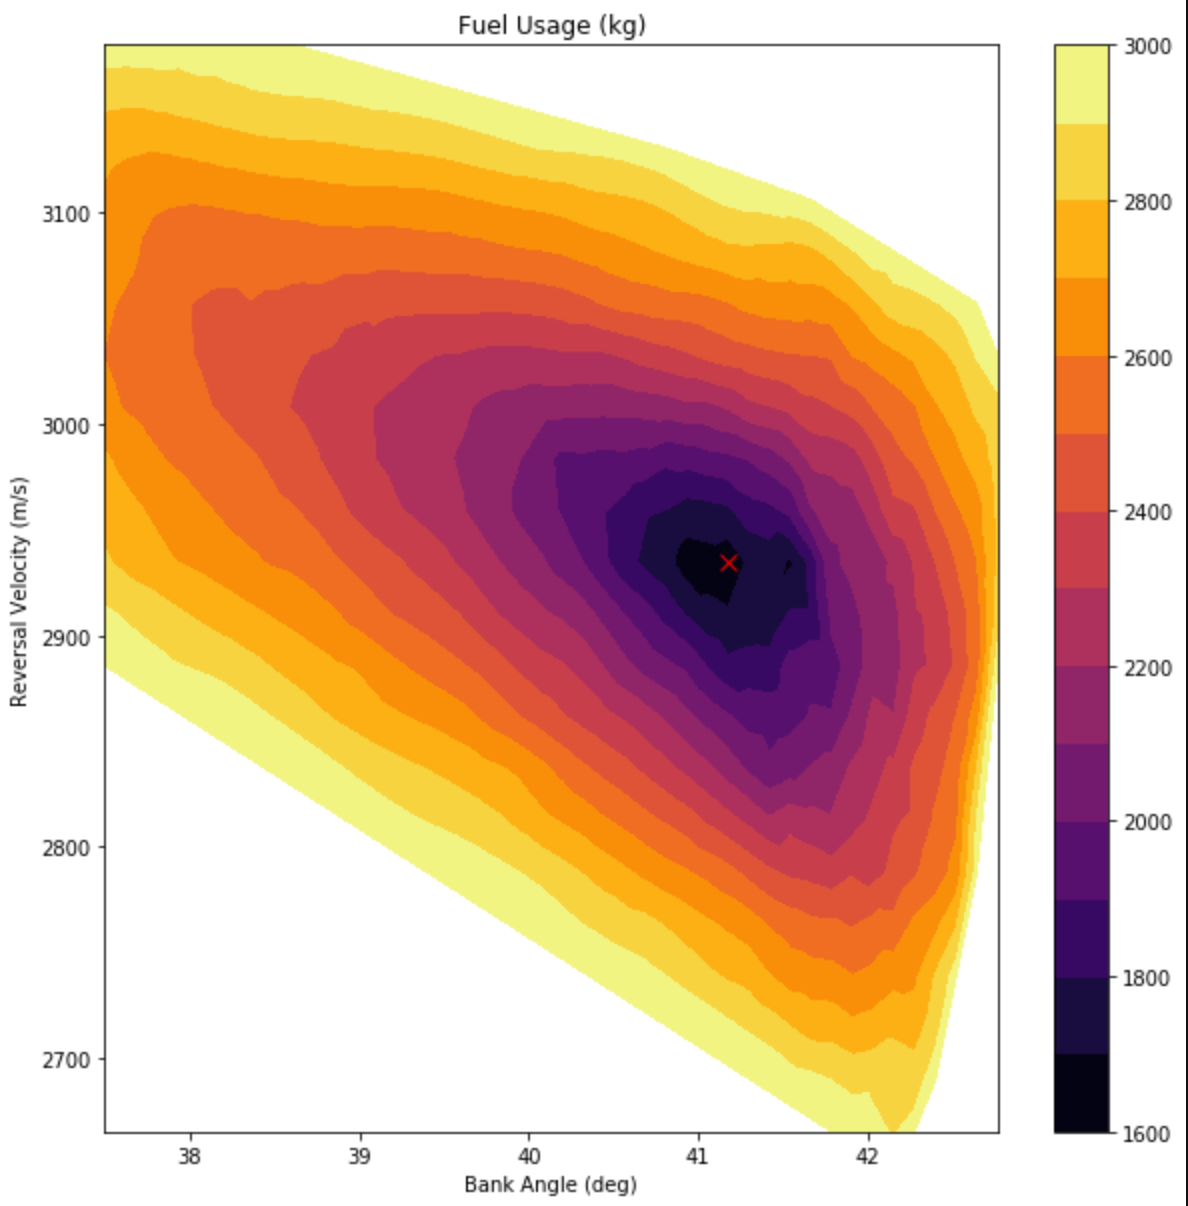
\includegraphics[width=0.9\textwidth]{Profile1_Objective} % first figure itself
		\caption{Contours of the objective function using a constant bank angle with one reversal}
	\end{minipage}\hfill
	\begin{minipage}{0.45\textwidth}
		\centering
		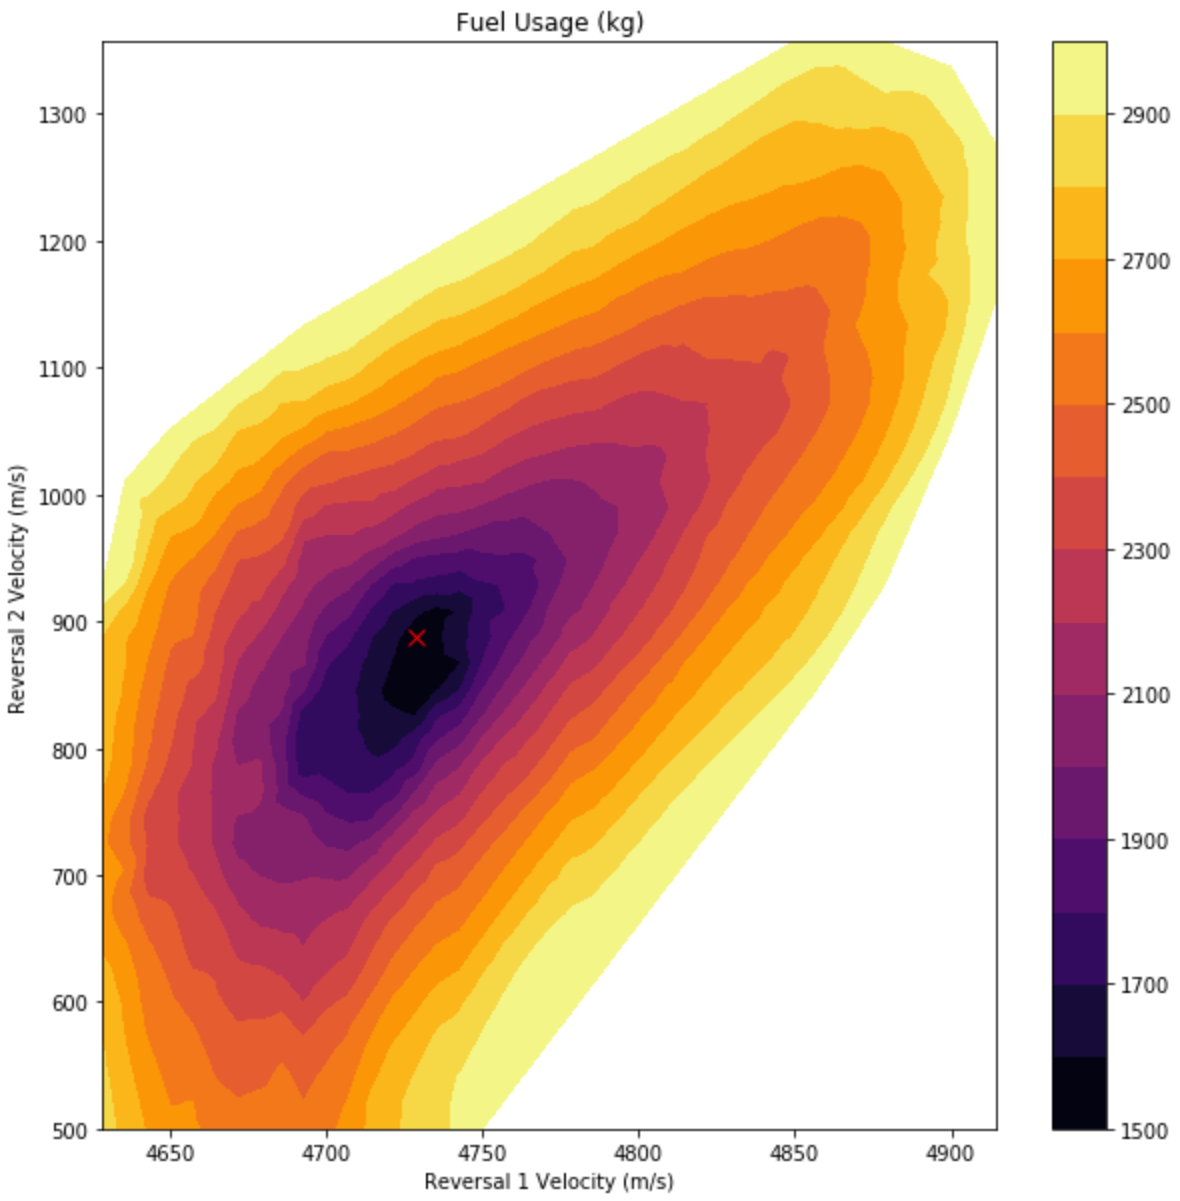
\includegraphics[width=0.9\textwidth]{Profile2_Objective} % second figure itself
		\caption{Contours of the objective function using the two reversal profile}
	\end{minipage}
\end{figure}

Each profile is capable of handling the $3\sigma$ entry flight path angle disturbances of $\pm 0.25^\circ$ when the nominal entry flight path angle and target downrange distance are chosen appropriately. It is possible to choose these values such that significant asymmetry exists. Surprisingly, the constant bank profiles require only about $5^\circ$ of variation to deal with this variation if known from the entry interface, and the reversal velocities require less than 100 m/s correction. 


%\begin{figure}[h!]
%	\centering
%	\includegraphics[scale=0.5]{"Profile1_Objective"}
%	\caption{Contours of the objective function using a constant bank angle with one reversal}
%\end{figure}

%The approach is very broad as it does not specify the entry parametrization to be used, the powered descent guidance, or how to compute the sensitivities required. 
% M2020 will fly Apollo EG and table GFOLD

%\section{Optimal Entry Trajectories}
%Similar to "Propellant Optimal Powered Descent Guidance" we will discuss several optimal control problems and their relationships. Each problem has the same objective of maximizing altitude at a fixed velocity, the constraints differentiate the problems. 
%
%Unconstrained Target Optimal Altitude Problem
%No constraint on terminal latitude/longitude, maximum velocity constraint, maximizing altitude. Entry flight path is free.
%
%No Crossrange Optimal Altitude Problem
%Terminal point must lie on great arc defined by the initial heading, maximum velocity constraint, maximizing altitude. Entry flight path is free.
%
%Fixed Target Optimal Altitude Problem
%Terminal point is fixed, entry flight path is free. 
%
%For these three problems, we have $h_{f_1} \ge h_{f_2}\ge h_{f_3}$. Observing the solutions to Problems 1 and 2, there is generally very little difference and the unconstrained terminal crossrange is less than 1 km for a variety of terminal velocities. 
%
%\section{Bank Angle Parametrization}
%Balancing computational complexity with expressiveness. What is the reachable set like? Even in predictor-corrector method where the bank angle is updated, a constant parametrization can still only predict performance as good as
%
%\section{Adaptive Powered Descent Initiation}
%Is the pinpoint landing problem monotonically decreasing in propellant? If not, how can we modify the problem to give us a suitable trigger? I would argue that downrange alone is not a suitable trigger since the crossrange and heading are also important. 



%\section{Apollo Entry Guidance}
%%Motivation: Near term missions using an adaptation of existing guidance with renewed purpose. M2020 will fly table GFOLD. 
%
%The venerated Apollo guidance flown during lunar return missions, adapted for Mars entry guidance, has been successfully demonstrated on the Mars Science Laboratory mission and is scheduled for use on the up and coming Mars 2020 entry capsule. The roots of the Apollo entry guidance can be traced back seven decades. Heritage is king in the aerospace industry where proven technologies are used until it is no longer possible, or a new enabling technology is required. For this reason, the Apollo entry guidance algorithm will be further modified to suit next generation needs for propellant optimal powered descent.

%\subsection{Existing Algorithm for Mars Entry Guidance}
%The modified Apollo guidance for Mars entry, termed in the Entry Terminal Point Controller (ETPC), relies on a reference trajectory to determine the feedback gains, or so-called influence coefficients, which are the sensitivities of the objective function to changes in the spacecraft state and control. The algorithm does not attempt to force the vehicle back to this reference, but instead seeks a suitable neighboring path that delivers the vehicle to the desired downrange distance at a fixed planet-relative velocity, based on the desired Mach number for parachute deployment. 
%
%% Math here, develop the form of the controller 
%More generally, any (first-order) ``terminal point" controller, i.e., one that seeks to drive the variation in a terminal objective $\phi: X\to\mathbb{R}$ to zero despite small variations $\Delta x$ in state/parameters from the reference, applies corrections to the nominal control computed via 
%\begin{align}
%\Delta u =  -\frac{\Delta \phi}{\lambda_u} =-\frac{\lambda_{\phi}^T\Delta x}{\lambda_u} 
%\end{align}
%where $\lambda_q(t) \triangleq \frac{\partial q(x(t_f))}{\partial x(t_f)}\frac{\partial x(t_f)}{\partial x(t)} $. Let $\Phi(t)\triangleq\frac{\partial x(t)}{\partial x(t_0)}$ denote the first-order state transition matrix (STM), computed along the nominal trajectory. Noting the following general relationship between adjoint (or reverse) sensitivities and forward sensitivities
%\begin{align}
%\lambda^T_{x}(t) &= \frac{\partial \phi(x(t_f))}{\partial x(t_f)}\Phi(t_f)\Phi^{-1}(t) \label{eq_stm_equivalence}
%\end{align}
%the control update can also be written in terms of the first-order state transition matrix 
%\begin{align}
%\Delta u(t) =  -\frac{\Delta x(t)^T \frac{\partial \phi(x(t_f))}{\partial x(t_f)} \Phi(t_f)\Phi^{-1}(t)}{\lambda_u(t)} 
%\end{align}
%
%
%Since the form of the controller is independent of the constraint, we need only update the constraint function to suit our needs, and all other aspects of the controller remain the same. 
%
%\subsection{Proof of Costate/STM equivalence, Equation {\ref{eq_stm_equivalence}}}
%\begin{proof}
%The STM is computed by solving initial value problem for the following variational equations
%\begin{align}
%\Phi (t_0) &= I \\
%\dot{\Phi}(t) &= \frac{\partial f}{\partial x} \Phi \label{eq_stm_ode}
%\end{align}
%while the adjoint is computed via backwards integration
%\begin{align}
%\lambda^T (t_f) &=  \frac{\partial \phi(x(t_f))}{\partial x(t_f)}\\
%\dot{\lambda}(t) &= -\frac{\partial f}{\partial x}^T \lambda \label{eq_adj_ode}
%\end{align}
%where the jacobian matrix in Eq.~(\ref{eq_stm_ode}) and (\ref{eq_adj_ode}) is evaluated along the reference trajectory.
%At the final time, we have 
%\begin{align}
%\frac{\partial \phi(x(t_f))}{\partial x(t_f)}\Phi(t_f)\Phi^{-1}(t_f) &= \frac{\partial \phi(x(t_f))}{\partial x(t_f)}\\
% &= \lambda^T (t_f)
%\end{align}
%Rearranging Eq.~(\ref{eq_stm_equivalence}) yields
%\begin{align}
%\lambda^T(t)\Phi(t) &= \frac{\partial \phi(x(t_f))}{\partial x(t_f)}\Phi(t_f)
%\end{align}
%where we note the right hand side is a constant value because $t_f$ is fixed. Differentiating both sides with respect to time yields
%\begin{align}
%\dot{\lambda}^T(t)\Phi(t) + \lambda^T(t)\dot{\Phi} (t)&= 0 \\
%-\lambda^T \frac{\partial f}{\partial x} \Phi + \lambda^T\frac{\partial f}{\partial x} \Phi&= 0 \\
%0 &= 0
%\end{align}
%which concludes the proof. 
%\end{proof}
%
%The terminal constraint must be altered because reaching a fixed downrange distance from the target at a fixed speed does not guarantee the spacecraft is in an optimal ignition condition as variations in the ignition flight path angle dictate that different downrange distances are optimal. Indeed, as \textbf{Ping Lu reference} rightly points out, no single state variable is an adequate indicator of a suitable ignition condition. To that end, we seek to define a terminal manifold such that any state lying on it represents an optimal ignition condition. In order to do so, we first develop the solution to a simpler propellant-optimal problem that admits a quasi-analytical solution. 
%
%\section{Fuel Optimal Braking}
%We proceed by recalling and extending results for propellant optimal braking, i.e., the problem of reducing the vehicle's velocity in a propellant-optimal way with no constraints on positional states. We consider the dynamics of a spacecraft in a constant gravity field written in Cartesian coordinates
%\begin{align}
%&\dot{x} = u \\
%&\dot{y} = v \\
%&\dot{z} = w \\
%&\dot{u} = \frac{T\cos\mu\cos\eta}{m} \\
%&\dot{v} = \frac{T\cos\mu\sin\eta}{m} \\
%&\dot{w} = \frac{T\sin\mu}{m} - g \\
%&\dot{m} = -\frac{T}{I_{sp}g_0}
%\end{align}
%with the objective $min_u J = \int_{t_0}^{t_f}T\, dt$ subject to a given initial condition and free final time. A terminal condition is applied only to the velocity components of the state. We assume without loss of generality that the target velocity vector is zero. The thrust magnitude is bounded $0 < T_{\min} \le T \le T_{\max}$. Let $X\in\mathbb{R}^7$ be the state vector, $U=[T,\,\mu,\,\eta]\in\mathbb{R}_+\times S^2$ and the equations of motion are expressed compactly as $\dot{X}=F(X,U)$. Denote by $P\in\mathbb{R}^7$ the vector of corresponding costates. 
%
%The Hamiltonian is $T + P^T\dot{X}$. The evolution of the costates is given by $\dot{P}=-P^T\frac{\partial F}{\partial X}$. Since there is no Mayer cost, a necessary condition for the costates corresponding to the states unspecified at the final time is $P_{x,y,z,m}(t_f)=0$. This implies the positional costates are identically zero over the whole trajectory, and the velocity costates are constant as a result. Primer vector theory indicates the optimal thrust direction is constant. Writing the Hamiltonian explicitly yields
%\begin{align}
%&H = T\left[1 + P_u\frac{\cos\mu\cos\eta}{m} + P_v\frac{\cos\mu\sin\eta}{m} + P_w(\frac{\sin\mu}{m} - g/T) - \frac{P_m}{I_{sp}g_0}\right] \\
%&\frac{\partial H}{\partial T} = 1 + P_u\frac{\cos\mu\cos\eta}{m} + P_v\frac{\cos\mu\sin\eta}{m} + P_w\frac{\sin\mu}{m}  - \frac{P_m}{I_{sp}g_0}
%\end{align}
%For the remaining analysis it is convenient to define $C = P_u{\cos\mu\cos\eta} + P_v\cos\mu\sin\eta + P_w\sin\mu$. Then, we can write
%\begin{align}
%\frac{\partial H}{\partial T} = 1 + \frac{C}{m}-\frac{P_m}{I_{sp}g_0} \\
%\dot{P}_m = \frac{TC}{m^2}P_m
%\end{align}
%from which is it clear that since $T>0,\, m>0,\,\mathrm{and}\, P_m(t_f)=0$, then $P_m$ is monotonic with the opposite sign as $C$. Furthermore, 
%\begin{align}
%\frac{d}{dt}\frac{\partial H}{\partial T} &= -\frac{C\dot{m}}{m^2}-\frac{\dot{P}_m}{I_{sp}g_0} \\
%&= \frac{CT}{I_{sp}g_0 m^2} - \frac{CT}{I_{sp}g_0 m^2} \\
%&=0
%\end{align}
%and thus the optimal thrust magnitude is constant. The magnitude depends on the sign of $C$. With constant thrust, this problem is equivalent to the minimum time problem, and the optimal thrust magnitude is always the maximum available. 
%
%With constant thrust magnitude and direction, the equations of motion can be solved analytically.  Define $k=\frac{T}{I_{sp}g_0}$ and the solution is
%\begin{align}
%&x(t) = x_0 + u_0t + \frac{T\cos\mu\cos\eta}{k^2}(m_0-kt)\log(1-\frac{k}{m_0}t)\\
%&y(t) = y_0 + v_0t + \frac{T\cos\mu\sin\eta}{k^2}(m_0-kt)\log(1-\frac{k}{m_0}t)\\
%&z(t) = z_0 + w_0t -\frac{1}{2}gt^2 + \frac{T\sin\mu}{k^2}(m_0-kt)\log(1-\frac{k}{m_0}t)\\
%&u(t) = u_0 + \frac{T}{k}\cos\mu\cos\eta\log(1-\frac{k}{m_0}t) \\
%&v(t) = v_0 + \frac{T}{k}\cos\mu\sin\eta\log(1-\frac{k}{m_0}t) \\
%&w(t) = w_0 + \frac{T}{k}\sin\mu\log(1-\frac{k}{m_0}t) -gt \\
%&m(t) = m_0 - kt 
%\end{align}
%
%Setting $u(t_f)=v(t_f)=w(t_f)=0$ results in three equations and three unknowns ($t_f,\, \mu,\, \eta$). Let 
%\begin{align}
%V_h &= \sqrt{(u(t_f)-u_0)^2 + (v(t_f)-v_0)^2} \\
%&= \pm\frac{T\cos\mu}{k^2}(m_0-kt_f)\log(1-\frac{k}{m_0}t_f) \label{eq_vh}
%\end{align} 
%where the sign ambiguity comes from having lost the sign of $u_0$. To resolve this we will assume $x_0 < 0$ and $u_0 > 0$. Then, Eq.~\ref{eq_vh} can be rearranged as $t_f = \frac{m_0}{k}\left(1-\exp(\frac{kV_h}{T\cos\mu})\right)$. 
%Dividing $gt_f-w_0$ by $V_h$ and solving yields $\mu = \tan^{-1}(\frac{-w_0 + gt_f}{V_h})$. Substituting this value of $ \mu $ into the expression for $t_f$ and simplifying yields the following equation
%\begin{align}
%t_f &= \frac{m_0}{k}\left[1 - \exp\left(-\frac{\sqrt{u_0^2 + v_0^2 + w_0^2 - 2V_hgt_f + g^2t^2_f}}{I_{sp}g_0}\right)\right] \\
% &= f(t_f)
%\end{align}
%which holds only for a unique value of $t_f$. Solving this transcendental equation for $t_f$ analytically does not appear possible. However, we can also view $f$ as a mapping that takes a value of $t_f$ and outputs an updated value. 
%\begin{theorem} \label{thm_tof}
%The sequence of times $\{t_n\}$ obtained by iterating with the previous result $t_n = f(t_{n-1})$ converges to a unique fixed point $t^*_f$, the optimal value of the time of flight, from any initial guess $t_0\in\mathbb{R}$.
%\end{theorem}
%\begin{proof}
%The range of $f$ is $[0, \frac{m_0}{k})$, attaining its lower bound only in the trivial case $u_0=v_0=w_0=t_f=0$, and bounded from above by the limit $\lim\limits_{t_f\to\pm\infty} =\frac{m_0}{k} $. 
%It follows that we need only consider its behavior on the interval $[0, \frac{m_0}{k})$, as any initial guess at $t_f$ (even a negative value) is immediately mapped to this interval. 
%
%Define the compact set $A=\{t\,|\,0\le t\le\frac{m_0}{k}\}$ and it follows $f(A)\subset A$. Let $d(x,y) = |x-y|$. Then $ (A,d) $ is a complete metric space. Recall that a function $f: A\to A$ is a contraction mapping on $A$ if there exists $c\in[0,1)$ such that $d(f(x),f(y)\le cd(x,y)$ for every $ x,y $ in $A$. Observe the following properties of $A$ and $f$ restricted to $A$:
%
%\begin{align}
%&\max_{a,b\in A} |a-b| = \frac{m_0}{k} \\
%&\max_{a\in A} f(a) = \frac{m_0}{k}\left[1 - \exp\left(-\frac{\sqrt{u_0^2 + v_0^2 +w_0^2 - 2V_hg\frac{m_0}{k} + g^2(\frac{m_0}{k})^2}}{I_{sp}g_0}\right)\right]  \\ % < \frac{m_0}{k}
%&\sup_{a,b\in A} |f(a)-f(b)| = |\max_{a\in A} f(a) - 0| = \max_{a\in A} f(a)
%\end{align}
%from which it follows that $f$ is a contraction mapping on $A$ with Lipschitz constant 
%\begin{align}
%c = 1 - \exp\left(-\frac{\sqrt{u_0^2 + v_0^2 +w_0^2 - 2V_hg\frac{m_0}{k} + g^2(\frac{m_0}{k})^2}}{I_{sp}g_0}\right) < 1
%\end{align}
%and, by the Banach fixed-point theorem, the result is proved.
%\end{proof} 
%
%Thus, $t_f^*$ can be determined simply by iterating. In practice, the iterates converge extremely quickly, obtaining millisecond precision within 5 iterations from a very poor guess such as a negative value, and 3 iterations from a more appropriate guess, such as that computed by assuming a constant mass. With $t_f$ known, the thrust angles are recovered via $\mu = \tan^{-1}(\frac{-w_0 + gt_f}{V_h})$, $\eta = \tan^{-1}(\frac{v_0}{u_0})$, and the complete solution to the propellant optimal braking problem is obtained. 
%
%\textit{Remark: Physically, if the ignition velocity is large enough, the vehicle will have insufficient propellant to decelerate. Mathematically, however, a solution always exists, including situations where the ignition velocity is impossibly high. Although intuitively it might seem not to be true, when the vehicle becomes nearly massless the thrust can decelerate the vehicle with incredible rapidity. In other words, any solution is guaranteed to satisfy $m(t_f)>0$ but not necessarily $m(t_f)\ge m_{dry}$.}
%
%\subsection{Analytical Solution}
%Although the development so far has needed no approximation, we have only achieved a quasi-analytical form due to the iteration required by Theorem~\ref{thm_tof} to find the time of flight. By introducing approximations that introduce very small errors, we can obtain a fully analytical solution. 
%
%	\begin{figure} 
%	\centering
%	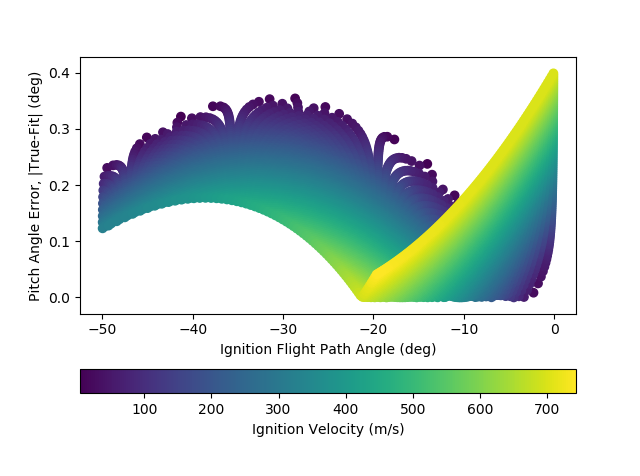
\includegraphics[width=4in]{pitch_angle_error_versus_fpa.png} 
%	\caption{\bf{Results of linear approximation to optimal pitch angle as a function of ignition flight path. The error is always smaller than $0.5^\circ$ over all ignition velocities and flight path angles of interest.}}
%	\label{fig_linear_fit}
%\end{figure}
%
%Solving the optimal control problem many times for a variety of initial velocities reveals the optimal thrust angle is extremely well-approximated as a linear function of the ignition flight path angle, i.e., $\mu = \mu_0 + a\gamma$. The optimal time of flight is then given by $t_f = \frac{V}{g}(\tan(\mu_0+a\gamma)  \cos\gamma - \sin\gamma)$. See Figure~\ref{fig_linear_fit}. Substituting this expression for the time of flight into the analytical expressions for the altitude and downrange distance flown as a function of time yields the optimal ignition altitude and distance. 
%
%Let the entry state vector be $x=[s, h, V, \gamma]$ and define 
%\begin{align}
%M(x) = \left[h - h^*(V, \gamma)\right]^2 + \left[s-s^*(V, \gamma)\right]^2 \\
%M(x) = \left[h + V\sin\gamma t_f -\frac{1}{2}gt_f^2 + \frac{T\sin\mu}{k^2}(m_0-kt_f)\log(1-\frac{k}{m_0}t_f)\right]^2 \nonumber \\
%       + \left[s + V\cos\gamma t_f + \frac{T\cos\mu}{k^2}(m_0-kt_f)\log(1-\frac{k}{m_0}t_f)\right]^2.
%\end{align} 
%The terminal manifold defining all propellant optimal ignition conditions is $\mathcal{M} = \{x\, |\, M(x)=0\}$. See Figure~\ref{fig_manifold} for a visualization of $\mathcal{M}$ with problem data: $m_0=8500$ kg, $g = 3.71\; \mathrm{m/s^2}$, $I_{sp} = 290$ s, $T_{\max} = 595$ kN. $M^{\frac{1}{2}}(x)$ is the distance between the spacecraft's current position and the optimal position corresponding to its current velocity. 
%
%	\begin{figure} 
%%	\centering
%	\includegraphics[width=6in]{manifold.png} 
%	\caption{\bf{The terminal manifold over $(V,\,\gamma)\in [0, 700]\times [-50^
%			\circ, 0^\circ]$. }}
%	\label{fig_manifold}
%\end{figure}
%	\begin{figure} 
%%	\centering
%	\includegraphics[width=6in]{manifold_single.png} 
%	\caption{\bf{The same terminal manifold with $V=600\, m/s,\;\gamma\in [-50^
%			\circ, 0^\circ]$. } Solutions demonstrate weak dependence of the optimal propellant expenditure on ignition flight path angle, with roughly 3\% variation over a $50^{\circ}$ change in $\gamma$.}
%	\label{fig_manifold_single}
%\end{figure}
%\subsection{Some Remarks on Fuel Optimal Braking}
%The solution to the propellant optimal braking problem was motivated by the need for an analytical representation of favorable ignition conditions for use in Apollo entry guidance. Targeting ignition conditions via this method does not preclude the use of a propellant optimal powered descent guidance with pinpoint landing capability, such as GFOLD. 

%Its relation to propellant optimal pinpoint landing. $J_{braking} \le J_{pp}$

%Compatibility with existing approaches (convex optimization, direct-method based, etc); simply tries to get the best condition possible and allows for more general profiles with optimal performance. Different triggering mechanism can be used (calling GFOLD)

%In a multi-phase optimal control formulation of the propellant-optimal pinpoint landing problem, the ignition condition always satisfied a constant maximal thrust, was the thrust angle also constant?


%\chapter{Fuel Optimal Feedback Control in One Dimension}
%A derivation for a one-dimensional soft landing of a vehicle in constant gravity, considering the effect of mass loss. The controller is first developed for a nominal system by solving an optimal control problem in feedback form. Then, the controller is modified to handle uncertainty and to reduce chattering. 
%
%\section{Equations of Motion}
%For the purpose of controller development, the dynamics governing the motion of the spacecraft are modeled as
%\begin{align}
%\dot{z} &= v \\
%\dot{v} &= \frac{T}{m} - g \\
%\dot{m} &= -\frac{|T|}{I_{sp}g_0}
%\end{align}
%where the spacecraft states $(z,\,v,\,m)$ are altitude, velocity, and mass, $g$ is a constant gravitational acceleration, $T$ is the thrust. We proceed by rewriting these equations in double integrator-like form via the following change of variables
%\begin{align}
%&x_1 = \frac{M}{T_{\max}}z  \label{eq_double_integrator}\\
%&\dot{x}_1 = x_2 =  \frac{M}{T_{\max}}v \\
%&\dot{x}_2= \frac{M}{m}u - \tilde{g}\\
%&\dot{m} = -k|u|
%\end{align}
%where $|u| \le 1$ is the control variable, $\tilde{g} = \frac{M}{T_{\max}}g$, $k = -\frac{T_{\max}}{I_{sp}g_0}$. $M$ is a upper bound on the initial mass value $\ge m_0$. The state vector is $x = [x_1,\, x_2,\,m]$.
%
%\section{Optimal Control Problem}
%We seek to minimize the propellant used to achieve a soft landing of the vehicle. We are interested in feedback solutions for their robustness, and because spacecraft rely on measured data. 
%\begin{align}
%\min_u J = \int_{0}^{t_f} |u| \mathrm{d}t \\
%x(0) = x_0 \\
%x(t_f) = 0
%\end{align}
%subject to the dynamic constraints, and $|u| \le 1$. The final time is free, as is the final mass. Naturally, the altitude must be positive everywhere except at the final time $x_1(t)\ge 0$, and the spacecraft carries a fixed amount of propellant $m(t)\ge m_{dry}>0$. For simplicity, we will consider only the cases without any upward velocity, $x_2(0)<=0$.
%
%
%\subsection{Analytical Solutions to EoM}
%For both powered and unpowered flight, we can solve the equations of motion analytically when the control is constant. This will be useful both in working with the necessary conditions for optimality, and for deriving the controller in state feedback form. We introduce the costates $p_{x_1}, p_{x_2}, p_m$, and the Hamiltonian for this problem is 
%\begin{align}
%H = |u| + p_{x_1}x_2 + p_{x_2}(\frac{M}{m}u-\tilde{g}) - p_mk|u|
%\end{align}
%and its partial derivatives with respect to the states and the control are
%\begin{align}
%&H_u = p_{x_2}\frac{M}{m} + (1 - p_mk)\mathrm{sign}(u) \\
%&H_{x_1} = 0 \\
%&H_{x_2} = p_{x_1} \\
%&H_m = -p_{x_2}\frac{M}{m^2}u
%\end{align}
%and it is noted that the Hamiltonian is a constant because it is not an explicit function of time.
%%from which we know that $p_{x_1}$ is constant, and $p_{x_2}(t) = p_{x_2}(0) - p_{x_1}t$. The Hamiltonian is a constant because it is not an explicit function of time. 
%The solution to the extended equations of motion in $\mathbb{R}^6$ determined by the Hamiltonian are:
%% However, we cannot solve explicitly the transcendental equations governing the time $t^*$ when $x_2(t^*) = 0$ due to a logarithmic term. Fortunately, the natural logarithm is well approximated by its Taylor series expansion near one. As a result, a second order expansion is conducted, and $t^*$ becomes the solution of a quadratic equation.  
%\subsubsection{Unpowered Case (U=0)} 
%\begin{align}
%&x_1(t) = x_1(0) + x_2(0)t - \frac{1}{2}\tilde{g}t^2 \\
%&x_2(t) = x_2(0) - \tilde{g}t \\
%&m(t) = m_0 \\
%&p_{x_1}(t) = p_{x_1}(0) \\
%&p_{x_2}(t) = p_{x_2}(0) - p_{x_1}t \\
%&p_m(t) = p_{m}(0)
%\end{align}
%
%\subsubsection{Powered Case (U=1)}
%\begin{align}
%&x_1(t) = x_1(0) + x_2(0)t - \frac{1}{2}\tilde{g}t^2 + \frac{M}{k}\left[t + (\frac{m(0)}{k}-t)\log(1-\frac{k}{m(0)}t)\right]\\
%&x_2(t) = x_2(0) - \tilde{g}t - \frac{M}{k}\log(1-\frac{k}{m(0)}t)\\
%&m(t) = m_0 - kt\\
%&p_{x_1}(t) = p_{x_1}(0) \\
%&p_{x_2}(t) = p_{x_2}(0) - p_{x_1}t \\
%&p_m(t) = p_{m}(0) + \frac{\frac{C}{m_0-kt}-\frac{C}{m_0}-p_{x_1}\log(1-\frac{k}{m_0}t)}{k^2}\\
%& C = -p_{x_1}m_0 + p_{x_2}(0)k
%\end{align}
%
%\subsection{Necessary Conditions}
%The control that minimizes the Hamiltonian is given by
%%\begin{align}
%%  u(t) = \left\{\begin{array}{lc}
%%        1, & \text{if } (1 - p_mk) + p_{x_2}\frac{M}{m} < 0\\
%%        -1, & \text{if } (1 - p_mk) - p_{x_2}\frac{M}{m} < 0\\
%%        0, & \text{otherwise. }
%%        \end{array} \right. % The period stops a warning about not closing the left 
%%\end{align}
%\begin{align}
%  u(t) = \left\{\begin{array}{lc}
%        1, & \text{if } 1 - p_mk + p_{x_2}\frac{M}{m} < 0\\
%        -1, & \text{if } p_mk - 1 + p_{x_2}\frac{M}{m} < 0\\
%        0, & \text{otherwise. }
%        \end{array} \right. % The period stops a warning about not closing the left 
%\end{align}
%
%\textbf{Next steps:} Prove the possible sequence of commands is $\{0,\,1\}$. Do this (perhaps) by first showing that only $u=1$ can be optimal at the final time. Then show this implies that $p_{x_1}>0$. Show that the switching curves are monotonic in time. 
%
%Claim: The control can only be $u=1$ at the final time. 
%
%Proof: Examine the $x_2$ equation for $u=0$. The spacecraft will reach zero velocity at $t=x_2(0)/g$ which is only a positive value for positive $ x_2(0) $. Thus there is no time such that $u=0$ will deliver the vehicle to the target conditions for the initial conditions under consideration. Similarly for $u=-1$, the vehicle's velocity is monotonically decreasing and thus can only reach zero from above. Recall from the problem statement that we consider only cases $x_2(0)<=0$. 
%
%%Proof 2: At the final time, $p_m=0$. 
%
%\textbf{The trivial case} $p_{x_2}(t_f)=0$ implies that either $p_{x_2}\ge0$, or it is identically zero for all time. We call this latter case the trivial case. If  $p_{x_2}(t)=0\,\forall t$, then $p_{x_1}=0$ as well. Additionally, this renders $p_m$ constant, and in fact it must be zero due to the necessary condition $p_m(t_f)=0$. Then the optimal control is $u=0\,\forall t$. The only initial states for which the terminal state constraints can be satisfied by this control are of the form $[0,\, 0,\, m_0]$ which trivially satisfy the constraints. Proof: Suppose a state $[z_0,\, v_0,\, m_0]$ exists such that $u=0$ will deliver it to the origin. Then, the final time is given by $t_f=v_0/g$ which is positive only for positive $v_0$, and $x_1(t_f) = 0 = z_0 + \frac{v_0^2}{2g} \implies z_0 = -\frac{v_0^2}{2g} <0 $ which contradicts our assumption that the initial altitude is positive. 
%
%%Claim: $p_{x_2}(t_f)<0$. Proof: Assume $p_{x_2}(t_f)\ge0$. We can dispense of the trivial case, leaving only the scenario that $p_{x_2}>0\,\forall\,t\not=t_f$. At the final time, for $u=1$, $1 + p_{x_2}\frac{M}{m}<0$ implies $p_{x_2}<0$ which contradicts our assumption.
%
%%Claim: The maximum number of switches is two. 
%
%%Claim: The sequence from -1 to 1 can never be optimal. Proof: Suppose this sequence is optimal. This would imply a time $\tau$ exists when $p_{x_2}(\tau)=0$ and $p_m(\tau)=k^{-1}$. However, $p_{x_2}=0$ implies that $p_m(t)=k^{-1}\,\forall t\in[\tau,\,t_f]$. This contradicts the necessary condition $p_m(t_f) = 0$.
%
%%Claim: The sequence from 1 to -1 can never be optimal. Proof: Suppose this sequence is optimal. This would imply a time $\tau$ exists when $p_{x_2}(\tau)=0$ and $p_m(\tau)=k^{-1}>0$. However, $p_{x_2}=0$ implies that $p_m(t)=k^{-1}\,\forall t\in[\tau,\,t_f]$. This contradicts the necessary condition $p_m(t_f) = 0$.
%
%%Claim: If the state and optimal costate are such that $u = 0$, there exists a positive time such that $(1 - p_mk) + p_{x_2}\frac{M}{m} = 0$. Proof: If $u=0$, then both $m$ and its costate are constant, and the condition becomes 
%%\begin{align}
%%(1 - p_m(0)k) + (p_{x_2}(0)-p_{x_1}t)\frac{M}{m_0} = 0
%%\end{align}
%%which can be solved for $t = \frac{\frac{m_0}{M}(1-kp_m(0))+p_{x_2}}{p_{x_1}}$. In order for this to be positive, the sign of $p_{x_1}$ must be the same as the numerator.
%%
%Two additional necessary conditions for an optimum are $H(t_f) = 0$ (which implies $H(t)=0\,\forall t\in[0,t_f]$ because it is constant), and $p_m(t_f) = 0$.
%Applying the latter to the former together with the requirement that $x_2(t_f)=0$ yields an algebraic relation between the final mass and the final costate $p_{x_2}$
%\begin{align}
%p_{x_2}(t_f) = \frac{|u|}{g-\frac{M}{m(t_f)}u}
%\end{align}
%From above we know that $ u $ must be positive at the final time and $p_{x_2}(t_f) = \frac{1}{\tilde{g}-\frac{M}{m}}<0$.
%%; however, we will prove this formally rather than rely on intuition. 
%%
%%\textbf{Case u = 0 at final time}
%%We find $p_{x_2}(t_f) = 0$ if $u=0$. This implies that either this costate is identically zero for all t, nonnegative for all t, or nonpositive for all t. 
%%
%%In the first case, $p_{x_1}=p_{x_2}=0$ and $p_m=$constant. For an optimum, $p_m(t_f)=0$ and thus all three costates are identically zero for all t. Then, the Hamiltonian for this problem is simply $H=|u|$ which is minimized by $u=0\,\forall\, t $. The only initial states for which the terminal state constraints can be satisfied by this control are of the form $[0,\, 0,\, m_0]$ which trivially satisfy the constraints. Proof: Suppose a state $[z_0,\, v_0,\, m_0]$ exists such that $u=0$ will deliver it to the origin. Then, the final time is given by $t_f=v_0/g$ which is positive only for positive $v_0$, and $x_1(t_f) = 0 = z_0 + \frac{v_0^2}{2g} \implies z_0 = -\frac{v_0^2}{2g} <0 $ which contradicts our assumption that the initial altitude is positive. 
%
%From the fact that $x_2$ is a linear function of time, we have $p_{x_1}=\frac{p_{x_2}(0)-p_{x_2}(t_f)}{t_f}$. Knowing that $p_{x_2}(t_f) < 0$ implies that either $p_{x_2}(0)\ge0$ and  $p_{x_1}>0$, or $p_{x_2}(0)<0$ and it is possible $p_{x_1} \le 0$. Claim: $p_{x_1} > 0$. Proof: Assume $p_{x_1} \le 0$. Then, $p_{x_2}(0) - p_{x_1}t \ge p_{x_2}(0)\,\forall\,t\ge0$. From the control that minimizes the Hamiltonian, if $u=0$, then it must be that 
%\begin{align}
%1-p_m(0)k+p_{x_2}(0) > 0 \\
%1-p_m(0)k+p_{x_2}(t) > 0 
%\end{align}
%which implies there is no $t_f\ge0$ such that $u=1$, but this contradicts $p_{x_2}(t_f) < 0$ (which is implied by $u=1$). %Additionally, it means that $p_m$ is constant, which contradicts the necessary condition unless it is identically zero for all t. 
%
%Knowing that $p_{x_1} > 0$, coupled with applying $H(t)=0$ with $u=0$ reveals that $p_{x_2}(t)=\frac{p_{x_1}x_2(t)}{g}$, thus $p_{x_2}(t)$ and $x_2(t)$ always have the same sign before the control is applied. Then, because upward velocities are disallowed, $p_{x_2}$ is strictly non-positive, and $u=-1$ can never be optimal. 
%
%Since $p_m$ is constant until the control is applied, it must tend toward zero once $u=1$ is applied to fulfill the necessary condition $p_m(t_f)=0$. Given that $x_2$ must tend toward zero from below, it follows that $p_m$ must decrease to zero, and therefore $p_m(0)>0$. More rigorously, when $x_2(t)\le0$, $p_{x_2}(t) \le 0$, and so $p_m$ is a strictly decreasing function of time for $p_{x_2}(t) \not= 0$, and thus $p_m(t)>0\,\forall t\in[0,\,t_f)$.
%
%%\textbf{Case u = -1 at final time}
%%$p_{x_2}(t_f) = \frac{1}{\tilde{g}+\frac{M}{m}} > 0$. 
%%If $p_m(0)$
%%sign($p_{x_2}$)=sign($\dot{p_m}$), so pm deriv can only change sign once. Pm is a parabola type thing as a result. 
%%Larger values of k actually encourage more thrust (presumably to end the hemorrhaging more quickly)
%
%
%\section{State Feedback Form}
%To determine the locus of points $(x_1(t),x_2(t), m_0)$ such that $u=1$, we first attempt to solve the velocity equation to find the time $t^*$ when it reaches zero:
%\begin{align}
%0 = x_2(0) - \tilde{g}t^* - \frac{M}{k}\log(1-\frac{k}{m(0)}t^*)
%\end{align}
%but this transcendental equation has no closed-form solution. Near unity, the natural logarithm has a convergent Taylor series; by constructing a second-order expansion of the logarithmic term, we obtain the following analytical approximation to $t^*$
%\begin{align}
%\tilde{t}^* = \frac{m^2(0)}{kM}\left(\tilde{g}-\frac{M}{m(0)} + \sqrt{(\frac{M}{m(0)}-\tilde{g})^2 - 2\frac{kM}{m^2(0)}x_2(0)}\right)
%\end{align}
%where we note that in solving the quadratic equation for $\tilde{t}^*$, it is always the positive branch that yields the positive root. Additionally, it is simple to verify that $\tilde{t}^* >= t^*$, i.e., $\tilde{t}^*$ is a conservative estimate of $t^*$ in the sense the vehicle will always reach zero velocity sooner than $\tilde{t}^*$, leaving the vehicle with some positive residual altitude. Thus, using $\tilde{t}^* $ in place of $t^*$ ensures no overshoot of the target altitude. 
%
%Proof: The Taylor series of the natural log around one is $\log(1-x)=-x-\frac{x^2}{2}-\frac{x^3}{3}-\dots$. The term $\frac{k}{m(0)}t \ge 0$, and therefore $-\log(1-x)\ge x+\frac{x^2}{2}\,\forall\,|x|<1$. Using the Taylor expansion results in an underestimate of the velocity reduction due to thrust, thereby resulting in an overestimate of the time to reach the target velocity. 
%
%All that remains to determine the (approximate) locus is to substitute  $\tilde{t}^* $ into the equation $x_1(t)=0$ and solve for $x_1(0)$ as a function of $x_2(0)$ and $m(0)$.
%
%%Note to self: The quasi-optimal controller uses a backoff (alpha) based on max disturbance based on gravity and mass loss. By incorporating these into the controller derivation, a much lower backoff can be used. 
%
%The optimal controller in state feedback form is given by
%\begin{align}
%u(x(t)) = \left\{\begin{array}{lc}
%1, & \text{if } x_1(t + \tilde{t}^*(x_2(t),m(t))) = 0\\
%0, & \text{otherwise. }
%\end{array} \right. % The period stops a warning about not closing the left 
%\end{align}
%
%\subsection{Example}
%The following parameters are assumed to compare nominal performance of three controllers: $T_{max}=4000\,N$, $g=1.62\, m/s^2$, k=$5.5\, kg/s$, and $x_0 = [4000c,\, -120c,\, 1050]$ where $c = 1050/4000$. The controllers under consideration are the propellant optimal controller derived above, the same controller but with $k=0$ essentially assuming a constant spacecraft mass, and final a robust quasi-propellant optimal controller that treats gravity and variable mass as disturbances with known bounds. 
%
%Figure~\ref{fig_compare_phase} shows the three trajectories through the phase space. From Figure~\ref{fig_compare_mass} it is clear that the derived controller performs best. Without knowledge of the mass dynamics, the derived controller expends more propellant, and produces undesirable high-frequency chattering as it slides along the switching surface. In contrast, the robust controller performs nearly as well despite knowing only bounds on the disturbance and without a significant reduction in chattering. In summary, the robust controller is capable but its downfall is treating gravity and mass dynamics as disturbances when they need not be. To that end, our next goal is to extend the derived optimal controller to the case with uncertain dynamics to enhance its robustness in the same manner.  
%
%
%	\begin{figure*} 
%	\centering
%	\includegraphics[width=4in]{compare_phase.png} 
%	\caption{\bf{Trajectories under three feedback controllers.}}
%	\label{fig_compare_phase}
%\end{figure*}
%	\begin{figure*} 
%	\centering
%	\includegraphics[width=4in]{compare_mass.png} 
%	\caption{\bf{Mass under three feedback controllers.}}
%	\label{fig_compare_mass}
%\end{figure*}
%	\begin{figure*} 
%	\centering
%	\includegraphics[width=4in]{compare_throttle.png} 
%	\caption{\bf{Throttle setting generated by three feedback controllers.}}
%	\label{fig_compare_control}
%\end{figure*}
%
%\section{Robustness to Unmodeled Disturbances}
%The tradeoffs between robustness and optimality are well known. In this section, we alter the control law to handle unmodeled disturbances of the form 
%$\dot{x}_2 = f(t, x, u) + \frac{M}{m}u - \tilde{g}$. The structure of the disturbance term $f$ may be very general in nature, capable of representing aerodynamic accelerations, gravity fluctuations, and state- and/or control- dependent stochastic variations.  We assume only that the disturbance has a known, finite upper bound $f \le f_{\max}$ satisfying $|f_{\max}|\le \frac{M}{m_0}-\tilde{g}$. Defining $G = - \tilde{g} - f_{\max}$, the above control law remains the same, only substituting $G$ everywhere that $\tilde{g}$ appears. 
%
%Notice that we do not require that $0 \le f_{\max}$, nor do we use its absolute value in defining $G$. This allows ``helpful" disturbances, such as atmospheric drag, to be handled without introducing conservatism due to neglecting their beneficial effects.  
%
%% A possible extension is to use a sliding mode observer (or other) to estimate the disturbance f, but will the algorithm tolerate time-varying g correctly? 
%
%% A possible extension is to assume a vanishing disturbance (like drag and gravity may be view as). Then, less conservative results may be obtained.  
%
%\section{Reduction of Chattering}
%The results of the previous section introduced robustness to the controller by preventing an overshoot of the switching surface due to disturbances. However, the resulting controller will chatter in an attempt to slide along the surface in the presence of disturbances. This can be alleviated at some cost to optimal performance by introducing a second switching surface and a memory term to the controller.
%
%\begin{align}
%u(x(t)) = \left\{\begin{array}{lc}
%1, & \text{if } x_1(t + \tilde{t}^*(x_2(t),m(t))) \le 0, u_{pre} = 0\\
%0, & \text{if } x_1(t + \tilde{t}^*(x_2(t),m(t))) \ge x_{BL}, u_{pre} = 1
%\end{array} \right. % The period stops a warning about not closing the left 
%\end{align}
%where $x_{BL}$ is a user defined boundary layer, $u_{pre}$ is the previous command which is initialized using the memoryless controller above, and updated each time the command changes. 
%







\end{document}